\chapter{Implementation of RoboMission}
\label{chap:implementation-of-robomission}

The first part of this chapter describes general aspects of the implementation,
such as used technologies and overall architecture of frontend and backend.
The second part presents a few selected details that are specific to the created system.

\section{System Architecture}

The application uses a standard client-server architecture,
with a fat frontend client communicating with server backend via REST API.
In addtion to the fronend app and backend service,
there are two other parts of the system:
scheduled jobs, which run periodically every night (e.g. metrics computation),
and tools for offline analysis of collected data
(jupyter notebook templates and helper functions).  % TODO: specify "helper functions"
% TODO: ref/cite human-in-the-loop principle
% TODO: other potential parts (future):
% - tasks/content management tools (CLI+browser)
% - simulations (CLI+browser)

% TODO: consider to include FE and BE sections below as subsections of this section

TODO: diagram of overall architecture (client-server, communication)

\section{Used Technologies}

Table \ref{tbl:technologies} shows overview of the tehcnologies used
in the project at the beginning of 2018.
Note that they are gradually evolving, either to meet new requirements,
or simply to replace old technologies with newer ones.
This is especially true for frontend, where the tools and best practices
are evolving rapidly.
When this project started in 2015,
we used several at that time popular technologies
(AngularJS, Bootstrap, bower, grunt)
which became obsolete during next 2 years,
so we replaced them by newer ones.
Many technologies were introduced naturally as the projects grew,
e.g. Django Rest Framework for REST API,
or redux-saga for cleaner handling of asynchronous side-effects
(instead of the originally used redux-thunk).


\begin{table}[h]
\begin{center}
\begin{tabular}{l l l}
\toprule
Area & Technology & Main Reason  \\
\midrule
Version control & git, GitHub & easy to use \\
Custom commands & make + django, npm & easy to use \\
Project management & GitHub (issues, project board) & easy to use \\
% Monitoring & Google Analytics & widely-used \\
\hline
\textbf{Backend} & Python 3 & concise, high-level \\
Dependencies & pip & easy to use \\
Environment & virtualenv[wrapper] & easy to use \\
Unit tests & pytest & concise, readable \\
Web framework & Django & feature-complete, well-documented \\
REST API & Django Rest Framework & feature-complete, well-documented \\
Database & PostgreSQL & widely used \\
Web server & Nginx + Gunicorn & widely used \\
Scheduled jobs & cron (+ django-crontab) & standard tool \\
Data Export & Django Rest Pandas & tranformations before export \\
\hline
\textbf{Frontend} & ES6 & concise and readable code \\
Dependencies & npm & easy to use \\
Bundling & webpack & feature-complete, widely used \\
Compling & babel & feature-complete, widely used \\
State & redux  & predictable behavior, testability \\
Side effects & redux-sagas  & readability, testability \\
Views & React & declarativness, reausability \\
Design (UI) & Material-UI & looks good \\
HTTP client & axios & based on promises \\
Code Blocks & Blockly & well-tested \\
Parsing & PEG JS & declarative rules \\  %(Parsing expression grammar) \\
Interpretation & JS-interpreter & stepping, custom hooks \\
Localization & react-intl & single place for all messages \\
\hline
\textbf{Analysis} & jupyter, pandas, sklearn & interactivity, high-levelness \\
Plotting & matplotlib, seaborn & powerful; results look good \\
%Machine learning & sklearn & powerful \\
%\hline
%\textbf{Analysis} & Python 3 & high-level, widely used \\
%Documents & jupyter notebook & interactivity \\
%DataFrames & pandas & feature-complete, well-documented \\
%Plotting & matplotlib, seaborn & powerful, looks good \\
%Machine learning & sklearn & powerful \\
\bottomrule
\end{tabular}
\end{center}
\caption{%
  Overview of main technologies used in the project. %
  The \emph{Reason} briefly explains why we have chosen the particular technoglogy
  (not why we have covered the area at all).}
\label{tbl:technologies}
\end{table}

\section{Frontend}

The frontend is a single page application with redux-architecture,
which means that there is a single state (model) storing all application data,
all the only way the state can be changed is by dispatching actions.
Each part of state then defines its reducer,
which is a pure function that takes previous state, action, and returns a new state.

TODO: redux-architecture diagram (specifically for our app)

TODO: show how the flow of events is easier to reason about in React+Redux (than in Angular)

\subsection{React Components}

\begin{itemize}
\item mostly declarative - simple mental model: rebuilding from scratch every time anything change -> less error prone
\item reusability -> use of single component on many places in different contexts,
  or even outside the app (use space-world for ai-search-workshop)
\item example from our codebase (code, image)
\end{itemize}

\subsection{Asynchronous Side Effects}

Frontend applications are usually full of asynchronous side effects
(e.g. fetching data from server, wating for user actions).
Many ways to handle them were proposed.
The most basic one are callbacks --
asychronous function takes a function (``callback'') as a parameter
and calls it once the asynchronous action is resolved.

(TODO: mention/explain promises -- advantage: very explicit; clean error
handling; show example for data fetching)

However, both callbacks and promises become awkward for expressing complex
asynchronous flows, such as visualizing code execution,
leading to unreadable ``callback hell''. % TODO: ref for callback hell
Sagas provide an alternative way of handling asynchronous effects using generators.
Instead of performing asynchronous effects directly, sagas yield
descriptions of such effects.
As an example, there is a saga responsible for processing
submitted feedback.
Note that while the code contains many asynchronous effects,
it can be read nearly as easy as standard linear synchronous code.

% TODO: insert comments in the code
% TODO: mention other advantage of sagas - great testability
% TODO: also mention new async-await concept

\begin{lstlisting}[language=ES6]
// Generator for single submit-feedback request
function* submitFeedback(action) {
  const { text, email } = action.payload;
  // Asynchronous request to get a value from state
  const url = yield select(getFeedbackUrl);
  try {
    // Asynchronous request to post data to server
    yield call(api.sendFeedback, url, text, email);
    // Asynchronous request to dispatch a new action
    yield put(actions.submitFeedback.success());
  }
  catch (error) {
    const { fieldErrors } = error;
    yield put(
      actions.submitFeedback.failure(fieldErrors));
  }
}
\end{lstlisting}


% TODO: add code samples for each concept (react component + image, reducer, saga)
% TODO(optional): awesome ES6 (example from our code)
% TODO(Material Design): example of our component + code

\begin{itemize}
\item TODO: (below) parsing task source, space world, robo code (PEG grammars)
\item TODO: Blockly
\item TODO: interpretation: saga + JS-interpreter
\end{itemize}

\section{Backend}

\begin{itemize}
\item Django, Django Rest Framework, (+ many small libraries, such as Django Rest Pandas)
\item django apps (python packages): learn, monitoring
\item models (...), serializers, views, services/use cases/core
\item data export
\item monitoring app, metrics computation
\item generators (e.g. metric computation)
\end{itemize}


\section{Monitoring and Analysis}

\begin{itemize}
\item monitoring dashboard etc. (! don't duplicate corresponding section in Design chapter)
\item Google Analytics, Feedback, Error reports
\item scheduled jobs -> compute metrics, export collected data
\item data export
\item pandas, (numpy, matplotlib, sklearn, seaborn)
\end{itemize}


\section{Tasks Description}

\begin{itemize}
\item in markdown (why)
\item online task editor
\item internal represenation (DB model and its serializers for FE and for CSV exports)
\item PEG grammars for whole task source, Space World (ref section below),
  and solution in RoboCode (ref section below)
\end{itemize}

Example of complete task source (for rendered task see figure \ref{fig:robomission-task1}. TBA: show rendered task and its source side by side)

\begin{lstlisting}
# turning-left
- category: moves

## Setting

```
|bM|b |b |bM|b |
|kA|k |kM|k |kA|
|k |k |kA|kM|k |
|kM|k |kS|k |kA|
```

## Solution

```python
left()
fly()
fly()
```
\end{lstlisting}


\section{SpaceWorld Grammar}

\begin{itemize}
\item TBA
\item together with RoboCode allows for a task sources in human-readable and editable markdown (TODO: insert example of space world and also of full task source with rendered game preview), and convenient online task editor
\end{itemize}


\begin{figure}[h]
\begin{center}
\begin{subfigure}{.4\textwidth}
\centering
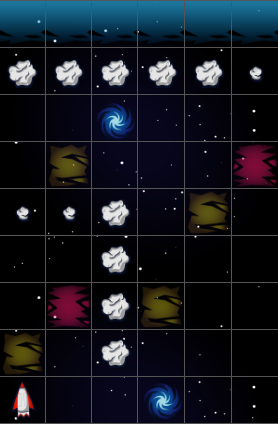
\includegraphics[width=.9\textwidth]{img/spaceworld}
\end{subfigure}
\begin{subfigure}{.36\textwidth}
\centering
{\lstset{numbers=none}
\begin{lstlisting}
|b |b |b |b |b |b |
|kA|kA|kA|kA|kA|kM|
|k |k |kW|k |k |k |
|k |y |k |k |k |r |
|kM|kM|kA|k |y |k |
|k |k |kA|k |k |k |
|k |r |kA|y |k |k |
|y |k |kA|k |k |k |
|kS|k |k |kW|k |k |
\end{lstlisting}}
\end{subfigure}
\end{center}
\caption{Example of Space World with its source code. TODO: Describe letters; consider replacing code listing with a screenshot from task editor with code highlighting}
\label{fig:spaceworld-source}
\end{figure}


\section{RoboCode}

\begin{itemize}
\item new programming language (RoboCode)
\item transformations (ast <-> RoboCode, MiniRoboCode, Blockly, JS)
\item common roboAST representation serves as a mediator between different languages
      that we need to support (Blockly for kids, RoboCode for writing,
      MiniRoboCode for logging, JS for running)
\item (allows for some cool magic such as immediate bidirecitional translating between blockly and RoboCode)
\item describe RoboCode PEG grammar and roboAST, iclude same example rules and parse trees
\item describe miniRoboCode format
\item describe RoboBlockly
\item describe RoboCodeJS
\item describe JS interpreter of RoboCodeJS
\end{itemize}

Example RoboCode, solution of the "Red Shooting" task (currently in figure: \ref{fig:spaceworld-source}), TBA: also include MiniRoboCode, JS, Blockly and AST for complete example.

\begin{lstlisting}
while color() != 'b':
    if color() == 'y':
        right()
    if color() == 'r':
        shoot()
    fly()
\end{lstlisting}
